%\input silabas.tex     % mis palabras separadas
\documentclass[12pt,doublespace,german]{report}
\input macros.tex       % mis macros que defino
\input paquetes.tex     % mis paquetes que uso
\input text_param.tex   % mis parametros de formato de tesis
\input espanol.tex      % texto renombrado a espanol

\numberwithin{equation}{section}

\begin{document}
	%\hyphenation{silabas}
	%\pagenumbering{roman} % numeracion de las primeras paginas
	%\thispagestyle{empty} % primera pagina sin numero

    %\input portada.tex    % la portada de tesis
    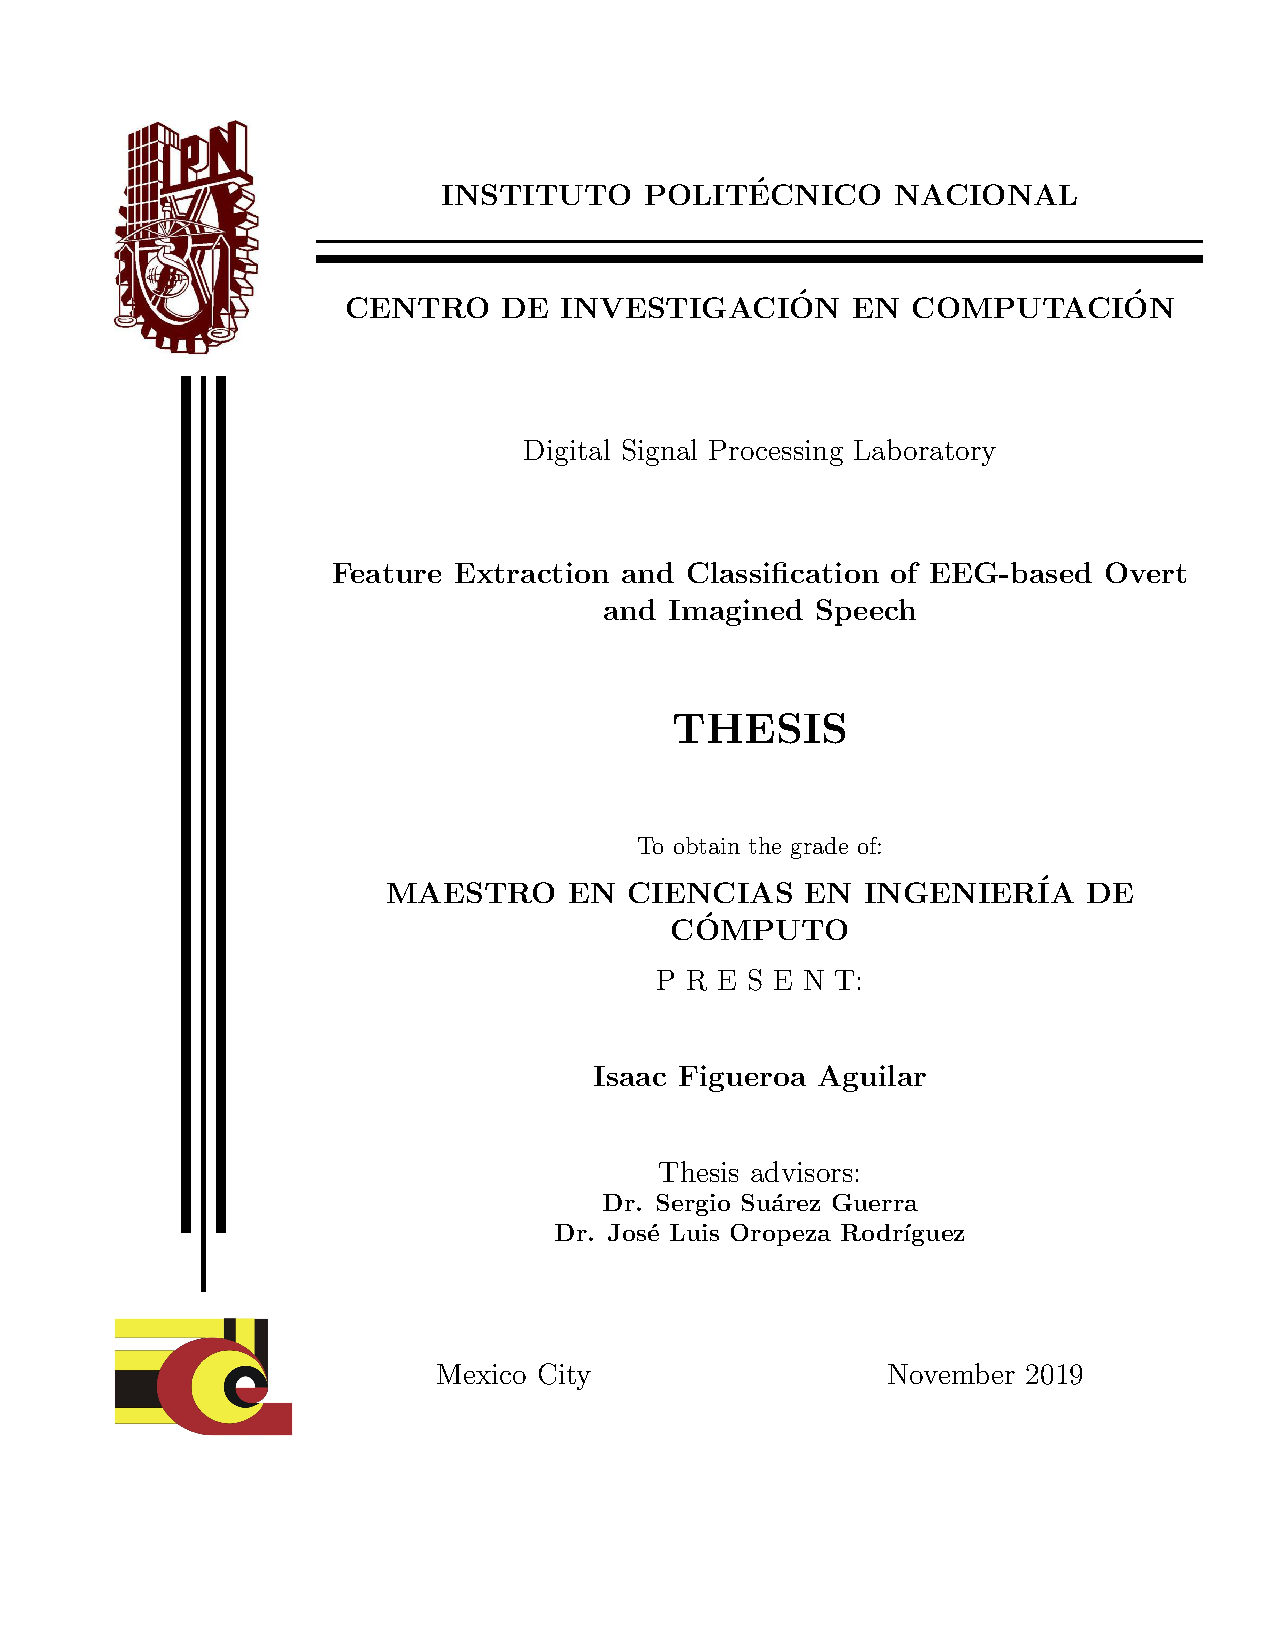
\includepdf{Documents/PortadaTesis.pdf}

   	\pagenumbering{roman} % numeracion de las primeras paginas
    %\input carta.tex
    \input thanks.tex

	%\def\tablename{Tabla} % cambia Table por Tabla.
	\def\listtablename{List of Tables}

	\tableofcontents      % crear indice de tablas
	\listoffigures        % crear lista de figuras
	\listoftables         % crear lista de tablas

	\baselineskip 2em     % 2em doble espacio, 1em espacio sencillo.

    %\input mgracias.tex   % agradecimientos especiales      % una cita cultural
    \input acronyms.tex
    \input glossary.tex
	\input resumen.tex    % resumen de la tesis en espanol
	\input abstract.tex   % resumen de la tesis en ingles
	\input chapter01.tex
	\input chapter02.tex
    \input chapter03.tex
    \input chapter04.tex
    \input chapter05.tex
    \input chapter06.tex
    \input chapter07.tex
    \input appendices.tex
    %\input {docs/CIEC_2011.pdf}
    \input references.tex
\end{document}

